\documentclass[aps,pre,twocolumn,superscriptaddress,nofootinbib,floatfix]{revtex4-2}
\usepackage{amsmath,amssymb}
\usepackage{graphicx}
\usepackage{booktabs}
\usepackage{bm}
\usepackage[colorlinks=true,linkcolor=blue,citecolor=blue,urlcolor=blue]{hyperref}
\newcommand{\dd}{\mathrm{d}}

\begin{document}

\title{Where forced defects go: corner charges, images and entropic screening in dimer coverings}

\author{Changyeon Won}
\email{cywon@khu.ac.kr}
\affiliation{Department of Physics, Kyung Hee University, Seoul 02447, Republic of Korea}

\date{Draft, \today}

\begin{abstract}
When a region cannot be covered completely by dimers, some sites must stay empty, and their position is decided by entropy alone. We show that this placement problem is two-dimensional electrostatics with three ingredients. A forced defect is a vortex of the height field whose winding equals the coordination number $z$. Every corner of the region carries a fixed fractional charge $q_c=-J_c/z$, set by the jump $J_c$ of the boundary height. A straight boundary produces images of the same sign. Together with the stiffness $g$ of the height field, these ingredients give the defect density in closed form, a single exponent formula for corners, edges and the interior, and a criterion for when a fixed charge binds a mobile defect. We test the framework with exact Pfaffian computations and Monte Carlo simulations in four ways. (i) On the square lattice, the same fixed charge that leaves a defect free in the interior binds it at an edge, because the image doubles the coupling. (ii) Varying $g$ twentyfold with interacting dimers, the edge and bulk pair exponents keep the predicted ratio $2.01\pm0.05$, and the corner exponent of a forced defect follows $g/2$. (iii) On the honeycomb lattice the winding is $3$. At $60^\circ$ corners the rule $q_c=-J_c/3$ holds as it stands. At $120^\circ$ corners it needs one new ingredient: the lattice boundary layer shifts the continuum boundary height by $\pm1/4$ on the two classes of armchair edges. A symmetry fixes the signs, and an exact infinite-strip calculation fixes the size to $3\times10^{-4}$. With this shift the theory reproduces full defect densities on hexagons to $3$--$6\%$ without fitting, and predicts the corner exponents of parallelograms blind. (iv) Breaking bipartiteness with diagonal bonds of weight $t$ screens the force beyond a length of order $1/t$. At the critical point $t=1/2$ the monomer pair correlation becomes a pure exponential, $[1-(\sqrt3-2)^{d}]/6$, because the underlying Toeplitz symbol becomes rational.
\end{abstract}

\maketitle

%==================================================================
\begin{figure*}[t]
\centering
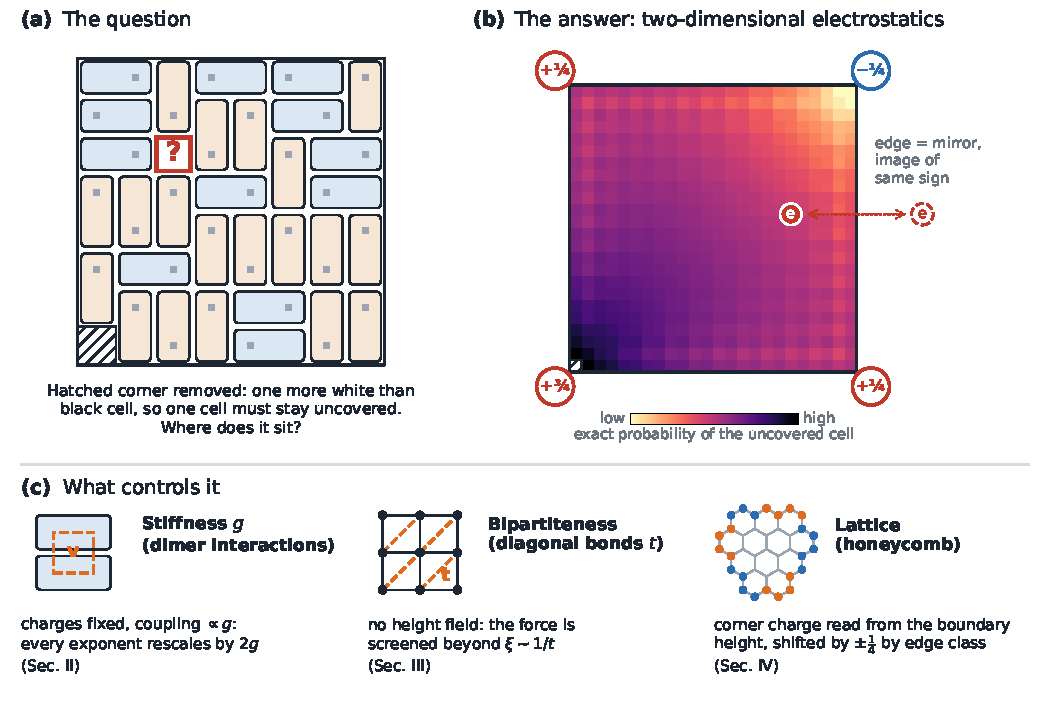
\includegraphics[width=0.95\textwidth]{figs/fig00_overview.pdf}
\caption{The problem and its electrostatic answer. (a) An $8\times8$ board with one corner removed has one more white than black cell, so every dimer covering leaves one white cell uncovered (a sample covering; grey squares mark black cells). Where is that cell? (b) Exact probability of the uncovered cell on a $24\times24$ board with the same corner removed. The cell is drawn to the removed corner and pushed away from the opposite one. This is what a charge $e=-1$ would do in the field of fixed charges at the corners ($q_c=+\tfrac34$ at the removed corner, $\pm\tfrac14$ at the others), with each edge acting as a mirror that makes an image of the same sign. (c) The three controls studied here: the stiffness of the height field, changed by interactions between dimers; bipartiteness, broken by diagonal bonds; and the lattice, changed to the honeycomb.}
\label{fig:overview}
\end{figure*}

\section{Introduction}
%==================================================================
Take a chessboard, remove one corner square, and cover the rest with dominoes [Fig.~\ref{fig:overview}(a)]. Since the board now has one more white square than black, one white square is always left uncovered. If all coverings are equally likely, where is that square likely to be? The answer is far from uniform [Fig.~\ref{fig:overview}(b)]. The empty square avoids the corner opposite the cut, is drawn to the cut, and its density near every corner and edge follows a power law whose exponent depends on the corner. Nothing in the problem has energy; every bias comes from counting coverings.

Questions of this kind arise whenever a constrained medium has to accommodate a defect it cannot remove. Examples are vacancies and holons in short-range resonating-valence-bond states and quantum dimer models~\cite{RokhsarKivelson1988,FendleyMoessnerSondhi2002,Henley2010}, the placement of unmatched sites in tilings with holes~\cite{Ciucu2010,Ciucu2017}, and the monomer-dimer problem itself~\cite{FisherStephenson1963,Kenyon2000,Alet2005}. In each case the defect is pushed and pulled by an entropic force, and the question is what determines that force near boundaries and corners, where real samples and finite flakes are always bounded.

The framework we use is the height (Coulomb-gas) description of close-packed dimers~\cite{Thurston1990,Nienhuis1984,Kenyon2000,Kenyon2001,Henley2010}. The constraint that every site be covered exactly once makes a height function well defined. Its long-wavelength fluctuations are those of a Gaussian free field with stiffness $g$, and a site left uncovered is a vortex of that field~\cite{FisherStephenson1963,Alet2005}. In the bulk this picture is rigorous: Ciucu proved that gaps in dimer coverings interact by two-dimensional electrostatics, first for lozenge tilings~\cite{Ciucu2010}, then on the square lattice~\cite{Ciucu2014,Ciucu2016} and on every doubly periodic bipartite lattice in the liquid phase~\cite{Ciucu2017}. Near a boundary, the image of a gap keeps its sign at constrained boundaries and reverses it at free ones~\cite{CiucuKrattenthaler2011,Ciucu2015,CiucuFischer2015}, and monomers on a straight boundary of the square lattice have exactly computable correlations~\cite{PriezzhevRuelle2008}. The jumps of the boundary height at corners were identified by Allegra as boundary-condition-changing operators~\cite{Allegra2015}, and the bulk monomer correlation has been obtained exactly even when bipartiteness is broken~\cite{FendleyMoessnerSondhi2002,BasorEhrhardt2007,BasorBleher2016}.

What is missing is a rule for the forced defect itself in a finite region: the field that the region's corners and edges exert on it, and how that field depends on the lattice and on the stiffness. Fig.~\ref{fig:overview}(b) suggests a simple answer. Every corner acts as a fixed fractional charge, $q_c=-J_c/z$, where $J_c$ is the jump of the boundary height at the corner and $z$ is the winding of a defect. Every straight edge acts as a mirror that produces an image of the same sign. For the square lattice at the free-fermion point, this rule reproduces exact defect densities on rectangles and on boards with removed corners to $1$--$3\%$ without adjustable parameters~\cite{PaperI}.

Here we derive the rule in a form that does not refer to any particular lattice, and test it in the three directions of Fig.~\ref{fig:overview}(c). Each test removes something the square-lattice case takes for granted. Section~\ref{sec:theory} sets up the electrostatics for a bipartite lattice of coordination $z$ and stiffness $g$. From it we derive a single exponent formula for a fixed charge at a corner, on an edge, or in the interior, and a criterion for binding. Section~\ref{sec:trap} tests the binding criterion exactly on the square lattice: the same charge binds a defect at an edge but not in the interior. Section~\ref{sec:g} changes the stiffness with interacting dimers and finds that all exponents scale together, as predicted. Section~\ref{sec:honey} moves to the honeycomb lattice, where the winding is $3$. There the corner rule survives but needs one new ingredient at $120^\circ$ corners, an edge-dependent shift of the boundary height that we determine by symmetry and an exact strip calculation. Section~\ref{sec:t} breaks bipartiteness and shows how the entropic force is screened. Section~\ref{sec:summary} collects what holds, what fails, and why.

%==================================================================
\section{Electrostatics of forced defects}
\label{sec:theory}
%==================================================================
\subsection{Heights, defects and corner charges}
Let the lattice be bipartite with sublattices black and white, and let every site have $z$ neighbours ($z=4$ on the square lattice, $3$ on the honeycomb). Thurston's height~\cite{Thurston1990} lives on the faces. Crossing an edge with a black site on the left, it changes by $+1$ if the edge is empty and by $-(z-1)$ if the edge carries a dimer. Around a covered site the changes add up to zero, so the height is single valued. Around an uncovered site they add up to $\pm z$, so a forced defect is a vortex of winding $z$. We give black defects the charge $e=+1$ and white defects $e=-1$.

Along the boundary of a simply connected region the height is fixed by the shape alone, since boundary edges cannot be crossed by dimers that leave the region. Along a straight edge it oscillates on the lattice scale but has a well-defined mean. At a corner the mean jumps by an integer $J_c$, defined modulo $z$ because the branch cut of a defect can be moved across the corner. The jumps around the boundary add up to $z$ times the net defect charge.

The jumps act as charges. In the upper half plane, the harmonic function with boundary value $0$ on $x<0$ and $J$ on $x>0$ is $(J/\pi)\arg z$. This is a vortex of winding $J$ over the half circle. A defect of winding $z$ sitting on a boundary with a same-sign image produces exactly the same function with $J$ replaced by $z$, since the defect and its image together wind by $z$ over the half circle. A jump $J_c$ is therefore equivalent to a fixed charge
\begin{equation}
q_c=-\frac{J_c}{z}
\label{eq:qc}
\end{equation}
at the corner, in units of the defect charge (the sign follows from orienting the boundary counterclockwise). The corner charges are fractional, depend only on the shape, and neutralize the defects: $\sum_cq_c=-\sum_ie_i$. On the board of Fig.~\ref{fig:overview}(b) the four corners of the full board carry $\pm\tfrac14$, and the removed corner becomes a corner of $+\tfrac34$.

\subsection{Density formula and exponents}
At long wavelengths the height is a Gaussian free field. We write its stiffness as $g$, normalized so that a pair of defects in the bulk correlates as $r^{-g}$; $g=1/2$ for non-interacting dimers on the square and honeycomb lattices, and $g$ is the same constant as in the Coulomb-gas analysis of interacting dimers by Alet \emph{et al.}~\cite{Alet2005}. A free boundary of the region is a Dirichlet boundary for the height, which makes images of vortices carry the same sign. Map the region conformally onto the upper half plane by $w=f(z)$, with the corners going to the real points $f_c$. The weight of a mobile defect of charge $e$ at $z$, in the presence of the fixed corner charges, is
\begin{equation}
\rho(z)\propto|f'(z)|^{g/2}(\operatorname{Im}f)^{g/2}\prod_c|f(z)-f_c|^{2g\,eq_c}.
\label{eq:rho}
\end{equation}
The first factor is the self-energy of the vortex, the second its interaction with its own image, and the product its interaction with the corner charges. Boundary charges coincide with their images, which doubles their coupling. A fixed charge $q$ in the interior at $f_q$ contributes $|f-f_q|^{g eq}|f-\bar f_q|^{geq}$ instead. At $g=1/2$ Eq.~\eqref{eq:rho} is the formula tested on rectangles in Ref.~\cite{PaperI}.

The exponent of the defect density near a fixed charge follows from the local form of $f$. Near a corner of interior angle $\theta$, $f-f_c\sim z^{\pi/\theta}$, so $\rho\sim d^{\gamma}$ at distance $d$ from the corner with
\begin{equation}
\gamma=2g\left[\frac{\pi}{\theta}\left(\frac12+eq\right)-\frac14\right].
\label{eq:gamma}
\end{equation}
A charge on a straight edge is the case $\theta=\pi$, $\gamma=2g(\tfrac14+eq)$, and a charge in the interior gives $\gamma=geq$ (Table~\ref{tab:gamma}). On a region of linear size $L$ the probability to find the defect within a fixed distance of the charge scales as $L^{-(2+\gamma)}$, and the corner-to-centre ratio as $L^{-\gamma}$.

\begin{table}[t]
\caption{Density exponent $\gamma$ near a fixed charge $q$ for a mobile defect $e$, $\rho\sim d^{\gamma}$. The defect is bound when $\gamma<-2$.}
\label{tab:gamma}
\begin{ruledtabular}
\begin{tabular}{lcc}
position & $\gamma$ & bound if \\ \hline
corner, angle $\theta$ & $2g[(\pi/\theta)(\tfrac12+eq)-\tfrac14]$ & $\gamma<-2$\\
straight edge & $2g(\tfrac14+eq)$ & $eq<-\tfrac1g-\tfrac14$\\
interior & $geq$ & $eq<-\tfrac2g$\\
\end{tabular}
\end{ruledtabular}
\end{table}

Two consequences are worth stating before the tests. First, $g$ enters Eq.~\eqref{eq:rho} only through the overall power, $\rho_g\propto\rho_{1/2}^{\,2g}$, because both the defects and the corner charges are vortices whose winding is fixed by topology. All exponents are therefore rescaled by the same factor. Second, the near-charge weight $\int d^{\gamma}\,d\,\dd d$ converges when $\gamma<-2$, and the defect is then bound to the charge with a probability that stays finite as $L\to\infty$. The edge exponent contains $2eq$ while the interior one contains $eq$: an image doubles the attraction. At $g=1/2$ a charge $eq=-3$ binds at an edge but not in the interior, and a single vacancy ($eq=-1$) binds at an edge for $g>4/3$ but in the interior only for $g>2$.

The assumptions are that the height has Dirichlet boundary conditions on free edges for all $g$, that no locking operator is relevant (which fails near the columnar transition of interacting dimers), and that the region is a flat liquid, i.e.\ its boundary does not force a nonzero tilt.

%==================================================================
\section{Fixed charges at an edge and in the interior}
\label{sec:trap}
%==================================================================
We first test the binding criterion where everything is exact: the square lattice at $g=1/2$. A fixed charge is made by removing cells. One removed black cell is a charge $q=1$. A plus-shaped hole (four black cells around a white one) is $q=3$. Two white cells removed far away restore the balance and leave one mobile white defect, $e=-1$. We place the fixed charge either at the centre of an $L\times L$ board or at the midpoint of an edge, compute the exact defect probability at every site with Kasteleyn matrices (Appendix~\ref{app:num}), and record the probability $P$ that the defect is within distance $3$ of the charge (Fig.~\ref{fig:trap}).

\begin{figure*}[tbp]
\centering
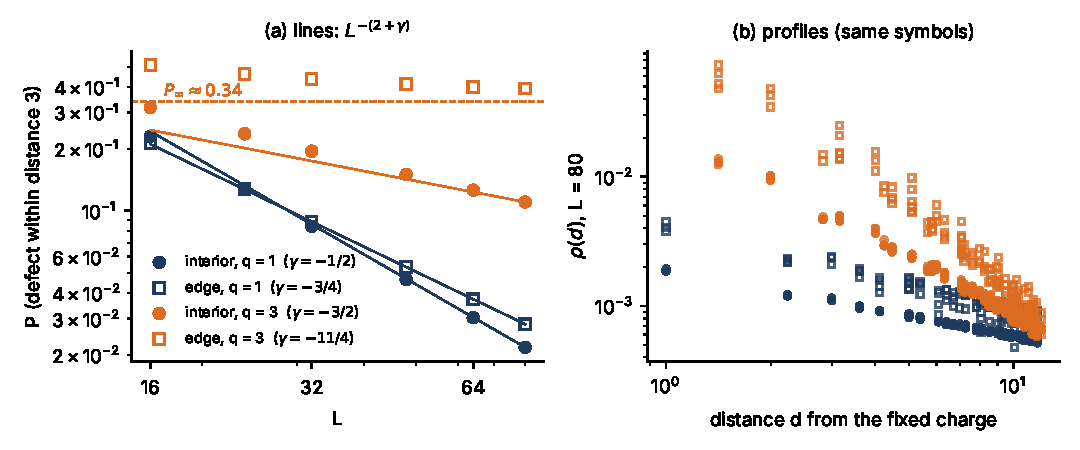
\includegraphics[width=0.9\textwidth]{figs/fig_trap.pdf}
\caption{A fixed charge in the interior and at an edge, square lattice, exact. (a) Probability that the mobile defect is within distance $3$ of the charge, against board size $L$. Lines show the predicted $L^{-(2+\gamma)}$. The edge charge $q=3$ is bound: $P$ tends to $P_\infty=0.34$ (dashed). (b) Density profile against distance from the charge at $L=80$.}
\label{fig:trap}
\end{figure*}

\begin{table}[t]
\caption{Fixed charges on the square lattice ($g=1/2$, mobile defect $e=-1$): predicted and measured scaling of the near-charge probability $P\propto L^{-(2+\gamma)}$ and of the profile $\rho\propto d^{\gamma}$, $L=16$--$80$.}
\label{tab:trap}
\begin{ruledtabular}
\begin{tabular}{lcccc}
charge & $\gamma$ & $P$: pred. & $P$: measured & profile \\ \hline
interior $q=1$ & $-\tfrac12$ & $L^{-1.50}$ & $L^{-1.44\ldots-1.48}$ & $-0.50$\\
edge $q=1$ & $-\tfrac34$ & $L^{-1.25}$ & $L^{-1.27\ldots-1.25}$ & $-0.68$\\
interior $q=3$ & $-\tfrac32$ & $L^{-0.50}$ & $L^{-0.72\ldots-0.60}$ & $-1.47$\\
edge $q=3$ & $-\tfrac{11}{4}$ & bound & $P_\infty=0.34$ & $-2.3$\\
\end{tabular}
\end{ruledtabular}
\end{table}

Table~\ref{tab:trap} shows the outcome. For $q=1$ the local slopes approach the predictions from both sides. For the interior $q=3$, the local slope drifts toward $-1/2$, and $P=aL^{-1/2}(1+b/L)$ fits all sizes to $0.7\%$; the profile slope $-1.47$ agrees with $-3/2$. The defect is not bound. The same hole placed on an edge binds it: $P=0.51,0.46,\dots,0.39$ for $L=16$--$80$ extrapolates to $P_\infty=0.34$. The edge profile is steeper than in the interior, as predicted, although with $\gamma=-11/4$ most of the weight sits within a few lattice spacings, where the continuum value is not reached. The image doubles the coupling, and the doubling is what turns a delocalized defect into a bound one.

%==================================================================
\section{Changing the stiffness}
\label{sec:g}
%==================================================================
Interactions between dimers change $g$ without changing the winding of the defects or the corner charges. We use the model of Alet \emph{et al.}~\cite{Alet2005}, with weight $e^{-\beta vN_\parallel}$, where $N_\parallel$ is the number of plaquettes holding two parallel dimers. Aligning interactions ($\beta v<0$) raise $g$ toward the columnar transition, and repulsive ones lower it. Equation~\eqref{eq:rho} predicts that every exponent is multiplied by $2g$. We test two consequences that have no free parameter.

\emph{Pair exponents.} A defect pair in the bulk decays as $d^{-g}$. A pair along a straight edge decays as $d^{-2g}$, because each defect interacts with the other's image as well. Their ratio is $2$ for every $g$. We sampled pair weights with a worm algorithm whose tail is fixed and whose head is the second defect, on a cylinder of circumference $64$ and height $128$. The tail is either in the bulk or on the open edge (Appendix~\ref{app:mc}). For $\beta v=+1,+0.5,0,-0.4,-0.7,-1$ the bulk exponent is $g=0.092$, $0.243$, $0.506$, $0.839$, $1.224$ and $1.880$ (exact $1/2$ at $\beta v=0$). The ratio of the edge exponent to the bulk exponent is $2.11$, $1.99$, $1.95$, $1.98$, $2.01$ and $2.00$, i.e.\ $2.01\pm0.05$ over a twentyfold change of $g$ [Fig.~\ref{fig:mc}(a,b)]. This also shows that the boundary condition stays Dirichlet, i.e.\ images keep their sign, at all $g$.

\emph{Corner exponent.} On an odd $L\times L$ board one black defect is forced, and each of the four corners carries $q_c=-\tfrac14$. Equation~\eqref{eq:gamma} with $\theta=\pi/2$ gives $\gamma=g/2$, so the corner-to-centre ratio decays as $L^{-g/2}$. Using an update that moves the defect itself (Appendix~\ref{app:mc}), we measured the ratio for $L=17$--$65$ [Fig.~\ref{fig:mc}(c)] and compared it with $g/2$, taking $g$ from the cylinder runs. For $\beta v=+0.5$, $0$, $-0.5$ and $-1$ we find $\gamma=0.116$, $0.239$, $0.461$ and $0.86$ from $L\ge25$, against $g/2=0.121$, $0.253$, $0.484$ and $0.940$ ($g$ at $\beta v=-0.5$ interpolated). The measured exponent tracks $g/2$ over an eightfold change of $g$. It lies $4$--$9\%$ below it, and the same offset appears at $\beta v=0$, where the exact value is $\tfrac14$; it comes from averaging over sites near the corner and decays slowly with $L$. The ratio $\gamma/g=0.47\pm0.01$ is therefore independent of $g$, as Eq.~\eqref{eq:rho} requires.

\begin{figure*}[tbp]
\centering
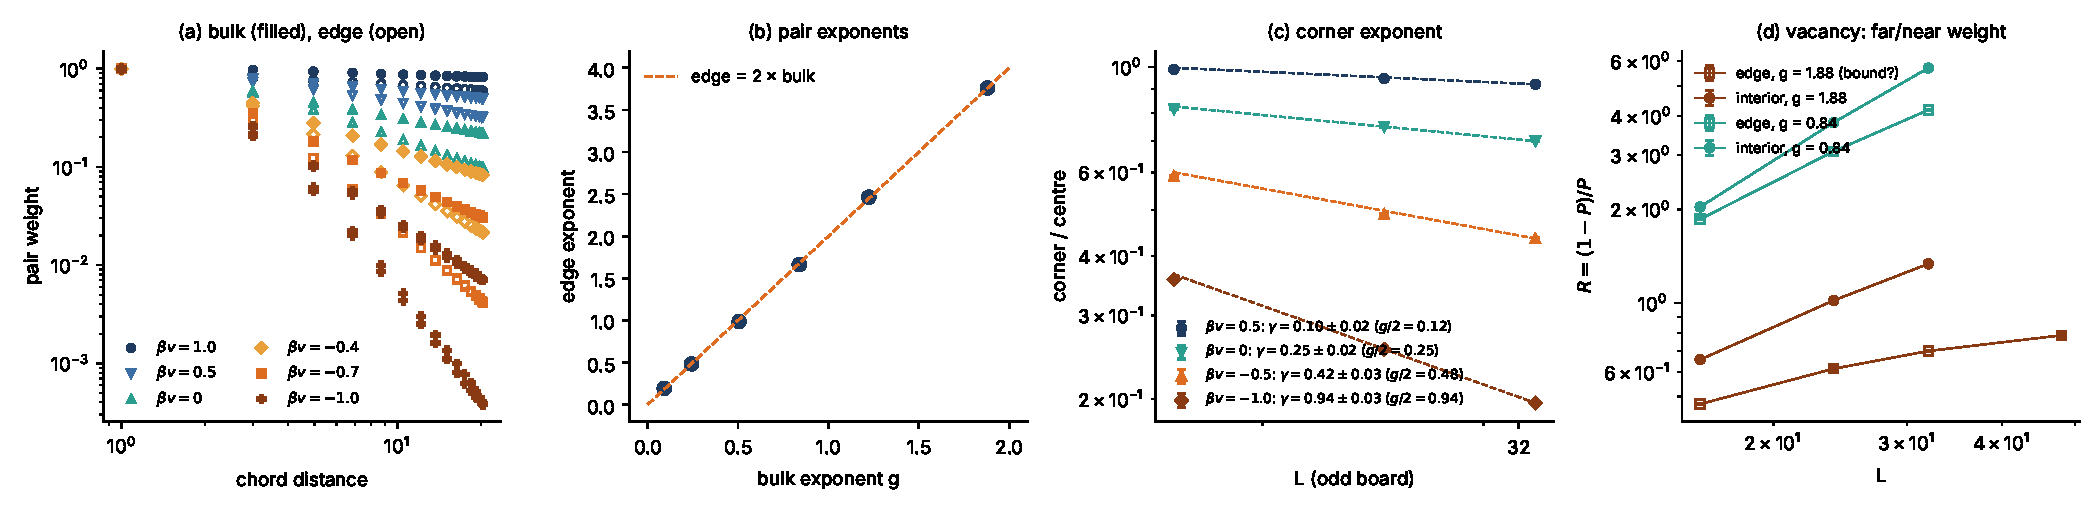
\includegraphics[width=0.98\textwidth]{figs/fig_mc.pdf}
\caption{Interacting dimers, Monte Carlo. (a) Pair weight against chord distance on a cylinder, with the tail in the bulk (filled) or on the open edge (open), for several $\beta v$. (b) Edge exponent against bulk exponent; the dashed line is $2g$. (c) Corner exponent of a forced defect on odd boards against $g/2$ (dashed).}
\label{fig:mc}
\end{figure*}

%==================================================================
\section{The honeycomb lattice}
\label{sec:honey}
%==================================================================
\subsection{Flat regions and forced defects}
Honeycomb dimers are lozenge tilings. A defect winds the height by $3$, so Eq.~\eqref{eq:qc} becomes $q_c=-J_c/3$, and $g=1/2$ as on the square lattice. This section tests whether the corner rule transfers to a lattice where corners come at two angles, $60^\circ$ and $120^\circ$.

The rule needs regions whose interior is a flat liquid. On the honeycomb this singles out armchair boundaries. Zig-zag regions are lozenge hexagons, which freeze near their corners into the arctic-circle shape~\cite{KenyonOkounkovSheffield}. Armchair flakes stay flat: the local deviation of the bond probabilities from $1/3$ decreases with size, and no bond is nearly frozen (Appendix~\ref{app:honey}, Fig.~\ref{fig:flat}). Armchair hexagons, triangles and parallelograms centred on an $A$ site have one more $A$ than $B$ site, so one $A$ defect ($e=+1$) is forced without removing anything (Fig.~\ref{fig:shapes}).

\begin{figure*}[tbp]
\centering
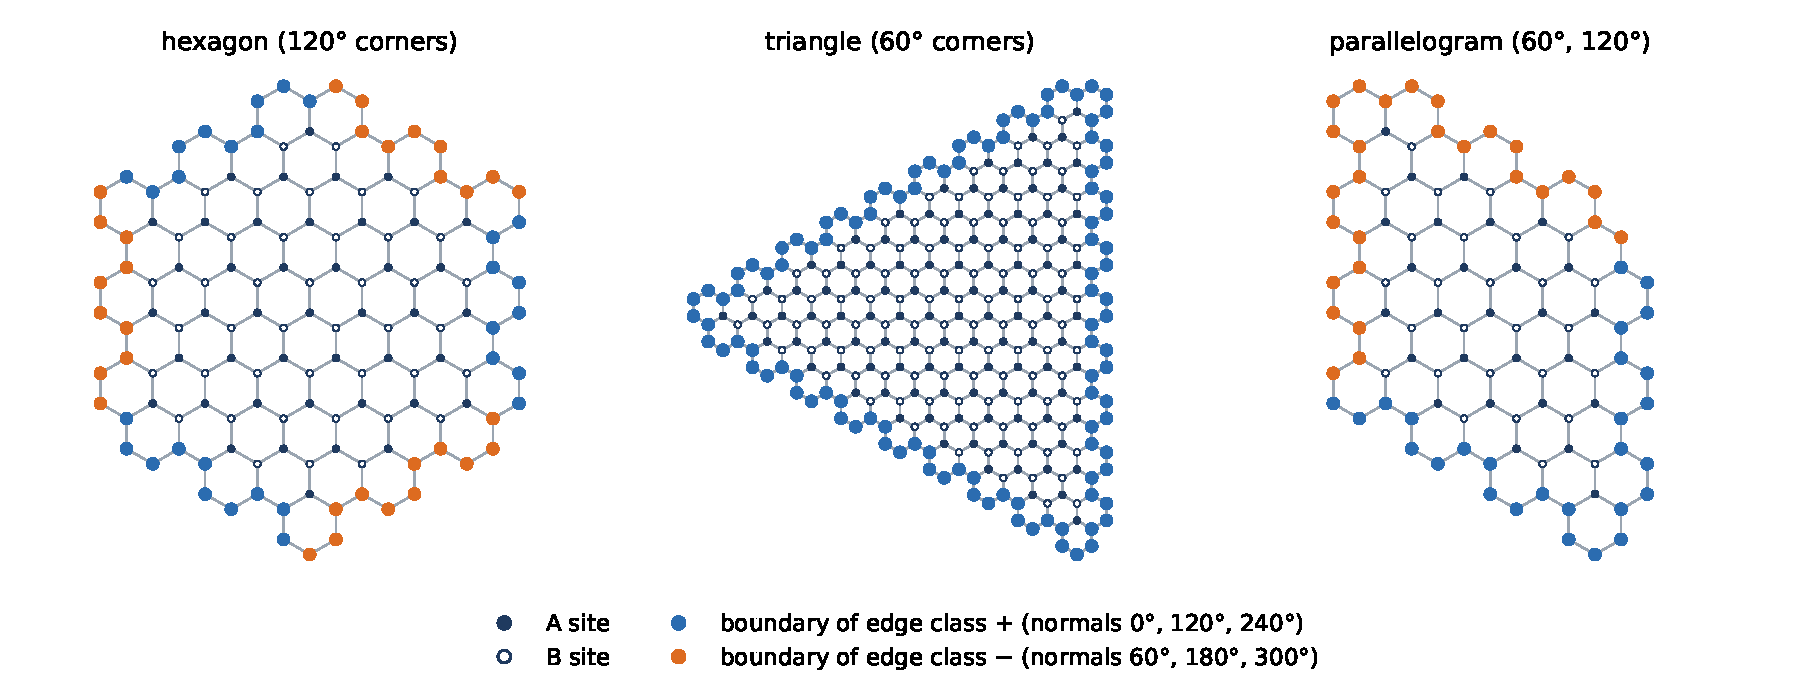
\includegraphics[width=0.9\textwidth]{figs/fig01b_honey.pdf}
\caption{Armchair regions on the honeycomb lattice, with boundary sites coloured by the class of their edge. Hexagons have only $120^\circ$ corners, each joining edges of different classes; triangles have only $60^\circ$ corners, joining edges of the same class; parallelograms have both.}
\label{fig:shapes}
\end{figure*}

Walking along the boundary on the dual lattice, the height steps by $+1$ or $-1$ depending on which sublattice lies inside. Along an armchair edge the steps alternate, so the mean height is constant and jumps only at corners (Appendix~\ref{app:honey}, Fig.~\ref{fig:height}). Hexagons fall into two families by how their corners terminate. Type I hexagons have $J=0$ and $+1$ on alternating corners, and type II have $J=-1$ and $+2$; in both $\sum_cJ_c=3$.

\subsection{$60^\circ$ corners: the rule holds as it stands}
Armchair triangles have three $60^\circ$ corners related by $C_3$ symmetry. Neutrality alone fixes $q_c=-\tfrac13$ at each, independent of any rule for $J$. The lattice jump is $J=+1$ at all three, so Eq.~\eqref{eq:qc} is exact here. Equation~\eqref{eq:gamma} with $\pi/\theta=3$ then gives $\gamma=\tfrac14$; without the corner charge it would be $\tfrac54$. We measure $\gamma=0.26\pm0.11$ from triangles of size $R=6$--$59$ [Fig.~\ref{fig:rule}(a)]. This geometry is of the type solved by Ciucu and Fischer~\cite{CiucuFischer2015}, whose ``zig-zag'' sides on the triangular lattice are our armchair edges. Their result corresponds to uncharged corners, and ours extends it to charged ones.

\subsection{$120^\circ$ corners: an edge-class shift}
On hexagons the rule fails. The corner exponents are $\gamma=0.28\pm0.02$ at both corners of type I and $0.75\pm0.07$ and $-0.25\pm0.02$ at the two corners of type II (Appendix~\ref{app:honey}, Fig.~\ref{fig:exponents}). Equation~\eqref{eq:qc} with the lattice jumps predicts $\tfrac12$ and $0$ for type I, and $1$ and $-\tfrac12$ for type II. It misses every $120^\circ$ corner by $1/4$ or more.

The missing ingredient is the boundary layer. The value of the height that enters the continuum theory is not the lattice boundary height, but the value the interior field extrapolates to at the edge. These can differ by a shift $\delta$ set on the lattice scale. Armchair edges come in two classes by the direction of their outward normal: $0^\circ,120^\circ,240^\circ$ (class $+$) and $60^\circ,180^\circ,300^\circ$ (class $-$). A $180^\circ$ rotation about the centre of a hexagonal face exchanges the two classes and the two sublattices, which reverses the sign of the height. Hence
\begin{equation}
\delta_-=-\delta_+ .
\end{equation}
A $60^\circ$ corner joins two edges of the same class and is unaffected. A $120^\circ$ corner joins edges of different classes, so its effective jump is $J\pm2\delta$.

The size of the shift follows from an exact calculation on an infinite armchair strip of half-width $R$ (Appendix~\ref{app:num}). The mean height has a linear interior profile, and extrapolating it to the two edges gives $\delta_--\delta_+$. The values are $0.402$, $0.484$, $0.489$, $0.505$, $0.502$, $0.4995$ and $0.5003$ for $R=12$, $20$, $40$, $60$, $120$, $240$ and $320$ [Fig.~\ref{fig:rule}(b)], within $2\times10^{-3}$ of $\tfrac12$ for all $R\ge80$. So $2\delta=\tfrac12$, and
\begin{equation}
q_c=-\frac{J_c+\sigma_c/2}{3}.
\label{eq:rule}
\end{equation}
Here $\sigma_c=+1$ ($-1$) if, going counterclockwise, the corner leads from a class $+$ (class $-$) edge to a class $-$ (class $+$) edge, and $\sigma_c=0$ at $60^\circ$ corners. In Allegra's language~\cite{Allegra2015}, the shift changes the boundary-condition-changing operator at a $120^\circ$ corner from the one set by $J$ to the one set by $J\pm\tfrac12$.

Equation~\eqref{eq:rule} gives $q_c=-\tfrac16$ at all six corners of a type I hexagon, hence $\gamma=\tfrac14$ everywhere. Type I hexagons are indeed Temperleyan~\cite{KenyonProppWilson}: all boundary $A$ sites have exactly the same defect probability, which requires equal charges at all six corners. For type II hexagons Eq.~\eqref{eq:rule} gives $+\tfrac16$ and $-\tfrac12$, i.e.\ $\gamma=\tfrac34$ and $-\tfrac14$. All four hexagon exponents now agree with the measurements within $1.5\sigma$.

\begin{figure*}[tbp]
\centering
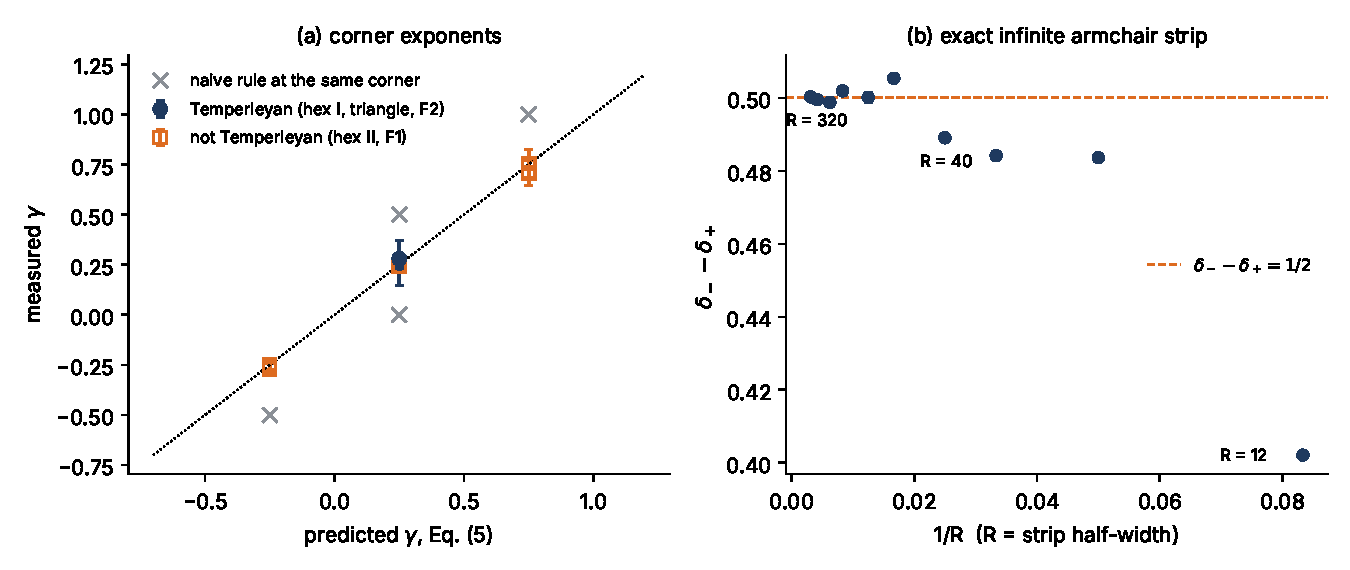
\includegraphics[width=0.85\textwidth]{figs/fig_honey_rule.pdf}
\caption{The edge-class rule on the honeycomb lattice. (a) Measured against predicted corner exponents for hexagons and triangles (calibration) and parallelograms (blind), with fit errors. Squares mark corners where the edge-class rule and the naive rule $q_c=-J_c/3$ agree; crosses show the naive prediction for the other corners. (b) Edge-class shift $\delta_--\delta_+$ from exact infinite strips against $1/R$; it tends to $\tfrac12$.}
\label{fig:rule}
\end{figure*}

\subsection{Full densities and a blind test}
Exponents probe the density only near corners. Equation~\eqref{eq:rho} predicts the whole density, so we compared it with exact densities on hexagons of both types. The map from the hexagon to the upper half plane is a Schwarz--Christoffel map (Appendix~\ref{app:num}), and the corner charges are taken from Eq.~\eqref{eq:rule} or from the lattice jumps. Nothing is fitted except the overall normalization. Figure~\ref{fig:hexdens} shows the profiles from the centre toward a $30^\circ$ corner, a $90^\circ$ corner and an edge midpoint. Away from the outermost three rows, the edge-class rule reproduces $\ln\rho$ with an rms deviation of $3$--$6\%$ on type I hexagons with $R=28,36$ and type II with $R=27,38$. The naive rule deviates by $7$--$14\%$, with systematic errors toward the corners. The result does not depend on whether the effective boundary is placed at the outermost sites or up to one lattice spacing outside.

\begin{figure*}[tbp]
\centering
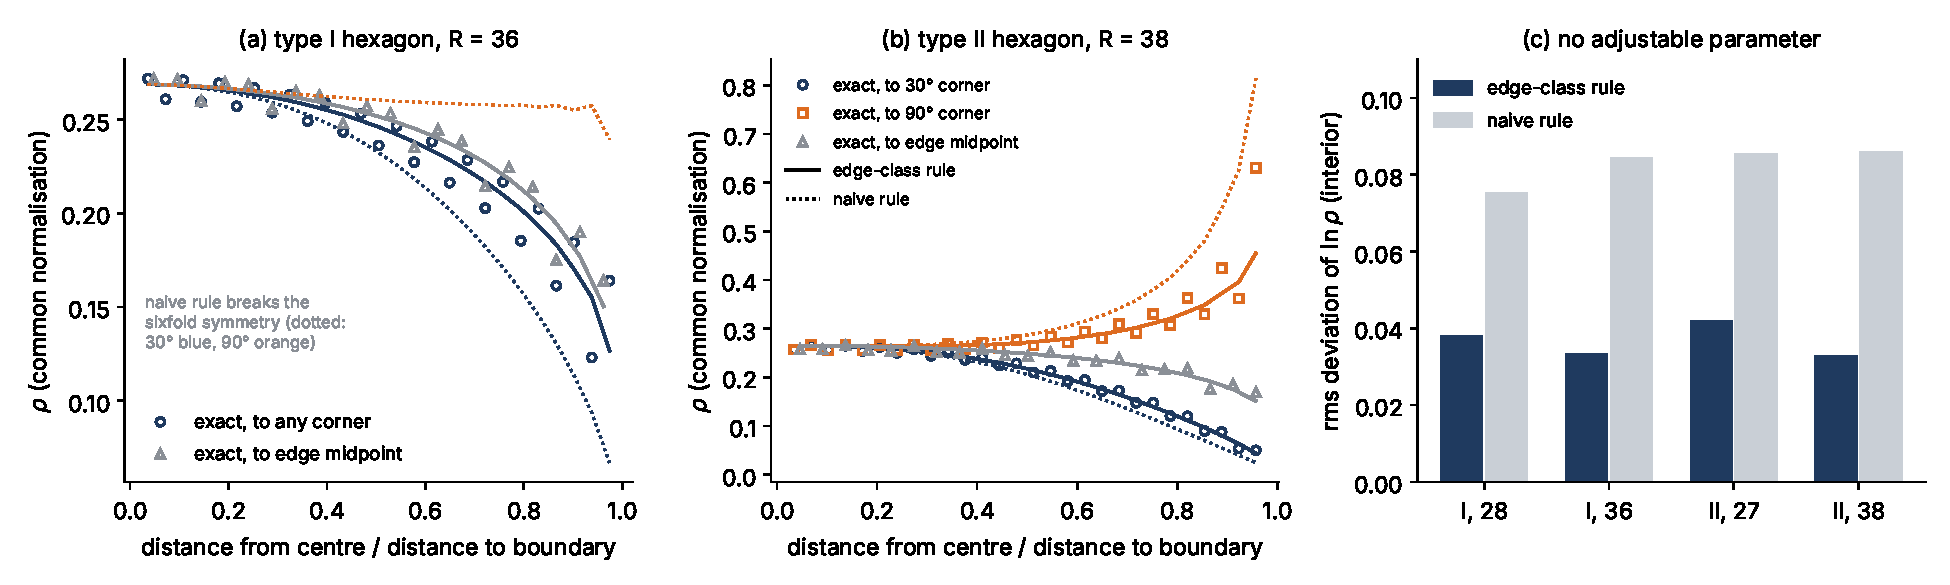
\includegraphics[width=0.98\textwidth]{figs/fig_hexdens.pdf}
\caption{Full defect density on armchair hexagons, exact (symbols) and Eq.~\eqref{eq:rho} with no adjustable parameter (lines). (a) Type I, $R=36$. (b) Type II, $R=38$. Solid lines use the edge-class rule, dotted lines the naive rule. (c) rms deviation of $\ln\rho$ over the interior for four hexagons.}
\label{fig:hexdens}
\end{figure*}

As a blind test we used armchair parallelograms, which have two $60^\circ$ and two $120^\circ$ corners. We fixed Eq.~\eqref{eq:rule} on hexagons and predicted the parallelogram exponents before computing them (Table~\ref{tab:para}). Of the eight corners, four discriminate between the rules: the $120^\circ$ corners at $30^\circ$ and $210^\circ$ in both families. All four lie within $1.2\sigma$ of the edge-class rule and $5$--$11\sigma$ away from the naive rule. The other four corners, where the rules coincide, agree as well.

\begin{table}[t]
\caption{Blind test on armchair parallelograms: predicted and measured corner exponents, with fit errors from the largest sizes. $J$ is the lattice jump with the branch cut at the $30^\circ$ corner. Asterisks mark the corners where the two rules differ.}
\label{tab:para}
\begin{ruledtabular}
\begin{tabular}{cccccc}
family & corner & $J$ & Eq.~\eqref{eq:rule} & naive & measured\\ \hline
F1 & $30^\circ$* & $-1$ & $+0.75$ & $+1.00$ & $+0.71\pm0.06$\\
F1 & $120^\circ$ & $+1$ & $+0.25$ & $+0.25$ & $+0.24\pm0.02$\\
F1 & $210^\circ$* & $+2$ & $-0.25$ & $-0.50$ & $-0.27\pm0.03$\\
F1 & $300^\circ$ & $+1$ & $+0.25$ & $+0.25$ & $+0.24\pm0.02$\\
F2 & $30^\circ$* & $0$ & $+0.25$ & $+0.50$ & $+0.28\pm0.02$\\
F2 & $120^\circ$ & $+1$ & $+0.25$ & $+0.25$ & $+0.28\pm0.02$\\
F2 & $210^\circ$* & $+1$ & $+0.25$ & $0.00$ & $+0.28\pm0.02$\\
F2 & $300^\circ$ & $+1$ & $+0.25$ & $+0.25$ & $+0.28\pm0.02$\\
\end{tabular}
\end{ruledtabular}
\end{table}

\subsection{Images on armchair edges}
At the midpoint of an armchair edge, a same-sign image predicts a defect probability $\propto R^{-1/4}$ relative to the centre and a profile rising as $d^{+1/4}$ into the bulk. An opposite-sign image would give $R^{+1/4}$ and $d^{-1/4}$. We find $R^{-0.29}$ (type I) and $R^{-0.24}$ (type II), and inward slopes $+0.20$ and $+0.21$ (Appendix~\ref{app:honey}, Fig.~\ref{fig:image}). Armchair edges are constrained boundaries in Ciucu's sense, for which images keep their sign~\cite{CiucuKrattenthaler2011,Ciucu2015}.

%==================================================================
\section{Breaking bipartiteness}
\label{sec:t}
%==================================================================
The height function exists only on bipartite lattices. To see what replaces the electrostatics when it does not exist, we add a bond of weight $t$ across one diagonal of every square plaquette [Fig.~\ref{fig:lattice}]. At $t=0$ this is the square lattice; at $t=1$ it is the triangular lattice. The graph stays planar, so Pfaffians remain exact (Appendix~\ref{app:num}).

\begin{figure}[t]
\centering
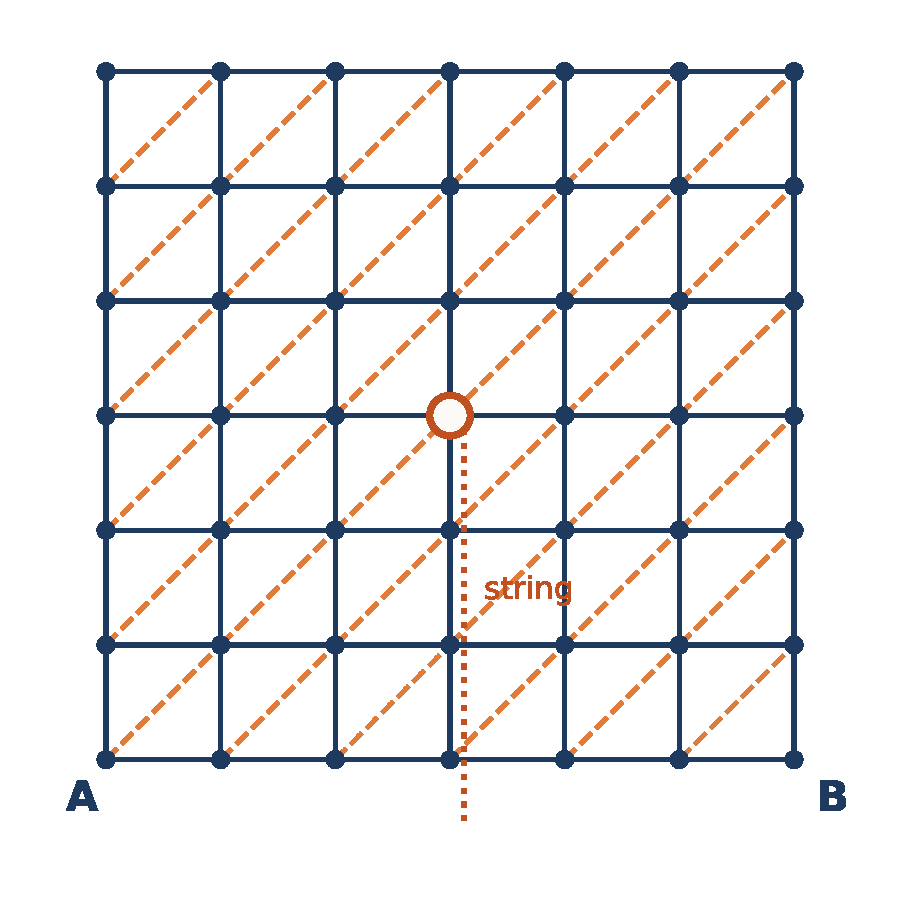
\includegraphics[width=0.62\columnwidth]{figs/fig01a_lattice.pdf}
\caption{Square lattice with diagonal bonds of weight $t$ (dashed). A defect (open circle) is attached to the boundary by a string (dotted) along which edge signs are reversed. The corners $A$ (touched by a diagonal) and $B$ become $120^\circ$ and $60^\circ$ corners of the triangular lattice.}
\label{fig:lattice}
\end{figure}

\subsection{Boundary trapping stops at $N\sim1/t$}
On odd $N\times N$ boards one defect is still forced. Figure~\ref{fig:ratio} shows the ratio $R$ of its probability at corner $A$ to that at the centre. At $t=0$ it decays as $N^{-1/4}$, the value $\gamma=g/2$ of Sec.~\ref{sec:g}. For $t>0$, $R$ saturates once $N$ exceeds roughly $1/t$, and the entropic force that held the defect away from the corner disappears. The saturated values depend on the corner angle (Table~\ref{tab:sat}): lattice-scale boundary information survives the screening.

\begin{figure}[t]
\centering
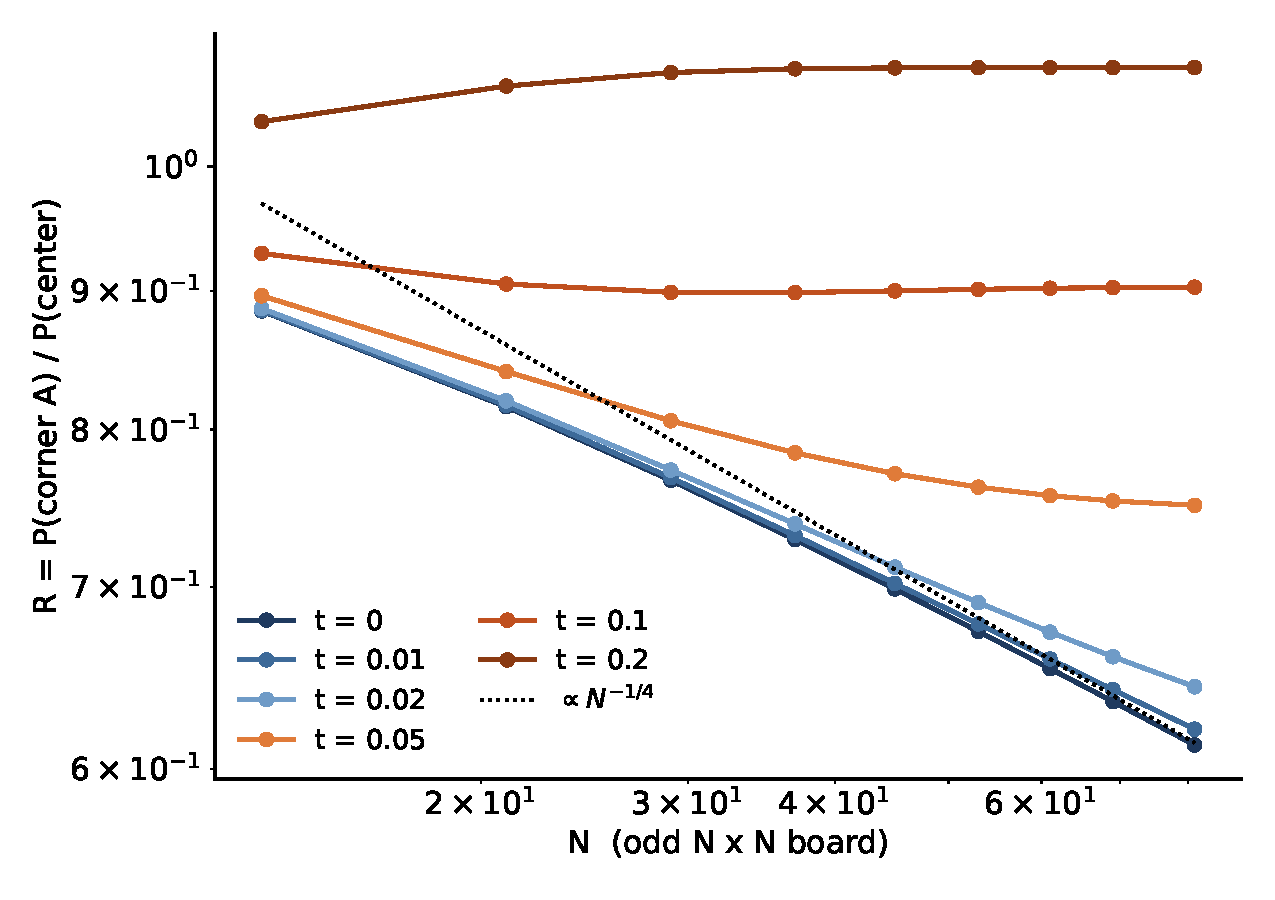
\includegraphics[width=0.95\columnwidth]{figs/fig02_corner_ratio.pdf}
\caption{Corner-to-centre ratio $R$ of a forced defect on odd $N\times N$ boards ($N\equiv1\pmod4$). At $t=0$, $R\propto N^{-1/4}$ (dotted); for $t>0$, $R$ saturates at $N\sim1/t$.}
\label{fig:ratio}
\end{figure}

\begin{table}[b]
\caption{Saturated corner-to-centre ratios $R_\infty$ ($N=61$).}
\label{tab:sat}
\begin{ruledtabular}
\begin{tabular}{ccc}
$t$ & corner $A$ ($120^\circ$) & corner $B$ ($60^\circ$)\\ \hline
0.2 & 1.087 & 1.172\\
0.5 & 1.350 & 1.732\\
1.0 & 1.526 & 2.587\\
\end{tabular}
\end{ruledtabular}
\end{table}

A naive scaling collapse, $R(N,t)/R(N,0)=G(N/\xi)$, gives an apparent $\nu\approx1.26$. The true value is $\nu=1$. Diagonal bonds join sites of the same colour, so once the defect is fixed the parity of the number of diagonal dimers is fixed, and $Z(-t)=\pm Z(t)$. Hence $\ln R(N,t)-\ln R(N,0)=a_2(N)t^2+O(t^4)$, and we find $a_2(N)=cN^2+eN\ln N+f$ with $c\approx0.015$ for both corners. The leading term $(Nt)^2$ is the one expected for $\nu=1$. The subleading coefficient is some thirty times larger than $c$, and it produces the apparent exponent. A fit on $N\le81$ predicts $a_2(101)$ to $0.1\%$, whereas a pure power law misses by $1.3$--$3.3\%$ (Appendix~\ref{app:t}).

\subsection{Pair correlations and the screening length}
In the bulk, the pair function $C(r)=Z(\text{two defects})/Z$ tends to a nonzero constant for $t>0$: the defects deconfine~\cite{FendleyMoessnerSondhi2002}. The limit $C_\infty(t)$ is known in closed form~\cite{BasorEhrhardt2007}, and its approach is $(-1)^{r+1}A\,r^{-1}e^{-2r\ln\eta_2}$ for $0<t<1/2$~\cite{BasorBleher2016}, with $\eta_2^{-2}=2-\mu-2\sqrt{1-t^2-\mu}$, $\mu=\sqrt{1-4t^2}$ and $\ln\eta_2=t+O(t^3)$. Our exact values up to $r=80$ reproduce $C_\infty$ to $10^{-13}$, the $r^{-1}$ prefactor, and the rate [Fig.~\ref{fig:pair}]. The screening length $1/(2\ln\eta_2)\simeq1/(2t)$ is the length at which the corner trapping above saturates.

\begin{figure*}[tbp]
\centering
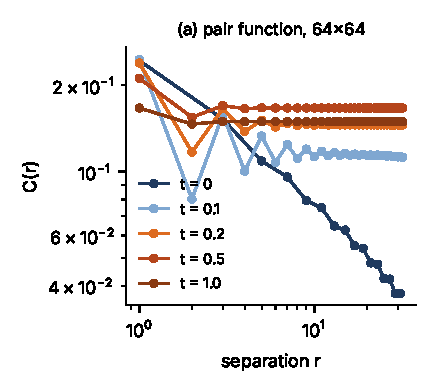
\includegraphics[width=0.33\textwidth]{figs/fig03a_pair.pdf}\hfill
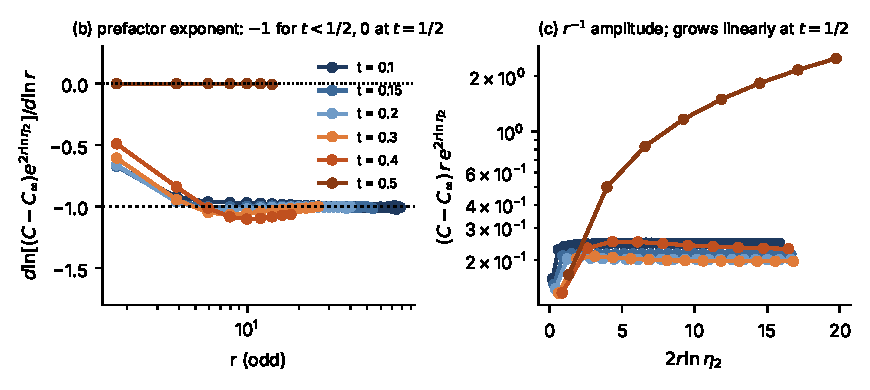
\includegraphics[width=0.64\textwidth]{figs/fig03b_mono.pdf}
\caption{(a) Bulk pair function $C(r)$ on $64\times64$ boards; at $t=0$ even separations vanish by the colour constraint. (b) Local prefactor exponent of $(C-C_\infty)e^{2r\ln\eta_2}$ (odd $r$); it tends to $-1$ for $t<1/2$ and to $0$ at $t=1/2$. (c) $(C-C_\infty)\,r\,e^{2r\ln\eta_2}$: flat for $t<1/2$, growing linearly at $t=1/2$ where the $r^{-1}$ prefactor is absent.}
\label{fig:pair}
\end{figure*}

\subsection{A pure exponential at $t=1/2$}
\label{sec:half}
The point $t=1/2$ is where the two rates $\eta_1,\eta_2$ of Basor and Bleher merge, and it is excluded from their theorems~\cite{BasorBleher2016}. There we find, to $10^{-10}$,
\begin{equation}
C(\Delta r,\Delta c)=\frac16\Bigl[1-(\sqrt3-2)^{|\Delta r|+|\Delta c|}\Bigr]\qquad(\Delta r\,\Delta c\ge0),
\label{eq:half}
\end{equation}
along $(1,0)$, $(0,1)$, $(1,1)$ and $(1,2)$ (Appendix~\ref{app:t}, Fig.~\ref{fig:half}); the anti-diagonal direction is different. The rate $\ln(2+\sqrt3)$ is the limit of $2\ln\eta_2$, and $C_\infty=1/6$ is the Basor--Ehrhardt constant. What is new is that the correction is a pure exponential at all distances. The structure of the symbol explains why. In the representation $C=\tfrac12\sqrt{\det T_n(\phi)}$ of Ref.~\cite{BasorBleher2016}, $\phi$ contains $[t^2+u+u^2]^{-1/2}$ with $u=\sin^2x$. For $t<1/2$ the two roots of $u^2+u+t^2$ produce square-root branch points, whose Fourier coefficients decay as $k^{-1/2}\eta_2^{-k}$ and give the $r^{-1}$ prefactor. At $t=1/2$ the roots merge, $u^2+u+\tfrac14=(u+\tfrac12)^2$, the square root disappears and the symbol becomes rational. For a rational symbol $\det T_n$ is a finite sum of exponentials. Evaluating the block determinant with $40$-digit arithmetic gives $C=[1-(\sqrt3-2)^{n+1}]/6$ for $n=1,\dots,30$ to $10^{-41}$, and $4C^2$ satisfies a linear recurrence of order three. Near $t=1/2$ the $r^{-1}$ form holds only beyond a crossover length $\propto(1/2-t)^{-1/2}$, which diverges at the critical point.

%==================================================================
\section{Discussion}
\label{sec:summary}
%==================================================================
The question of where a forced defect goes has a short answer on bipartite lattices: it goes where a charge $e$ would go in the field of fractional corner charges $q_c=-J_c/z$, with straight edges acting as same-sign mirrors and the stiffness $g$ setting the overall power. Table~\ref{tab:verdict} lists what we tested and the outcome.

\begin{table*}[t]
\caption{Tests of the electrostatic picture in this work.}
\label{tab:verdict}
\begin{ruledtabular}
\begin{tabular}{p{3.6cm}p{5.0cm}p{8.2cm}}
ingredient & prediction & outcome\\ \hline
image doubling at edges & binding at an edge for $eq<-\tfrac1g-\tfrac14$, in the interior for $eq<-\tfrac2g$ & square lattice, exact: $eq=-3$ bound at an edge ($P_\infty=0.34$), free in the interior; $q=1$ exponents within $0.03$\\
stiffness & every exponent $\propto2g$ & edge/bulk pair ratio $2.01\pm0.05$ for $0.09\le g\le1.9$; corner exponent tracks $g/2$ for $0.24\le g\le1.9$, $\gamma/g=0.47\pm0.01$\\
winding $z$ & $q_c=-J_c/z$ & honeycomb $60^\circ$ corners: $\gamma=0.26\pm0.11$ vs $\tfrac14$\\
boundary layer & non-universal & honeycomb $120^\circ$ corners need an edge-class shift $\pm\tfrac14$ (sign by symmetry, size from exact strips); full densities to $3$--$6\%$; blind parallelogram test passed\\
image sign & set by the boundary type & same sign on armchair edges, as for constrained boundaries~\cite{CiucuKrattenthaler2011,Ciucu2015}\\
bipartiteness & needed for the height & broken: trapping saturates at $N\sim1/t$ with angle-dependent limits; pure exponential at $t=1/2$ from a rational symbol\\
\end{tabular}
\end{ruledtabular}
\end{table*}

Two points deserve comment. First, the corner charge is a topological quantity only up to the boundary layer. On the square lattice the lattice jump and the continuum jump coincide. On the honeycomb they differ at $120^\circ$ corners by a fixed amount, $\pm\tfrac12$, which comes from the two edges meeting there rather than from the corner itself. Symmetry fixes its sign, and an exact strip calculation fixes its size. A closed-form evaluation of $2\delta=\tfrac12$, presumably through a Wiener--Hopf factorization of the strip problem, is left open; the Temperley property of type I hexagons shows that the value must be exactly $\tfrac12$. Second, the binding criterion separates edges from the interior through the image alone. For interacting dimers it predicts that a single vacancy binds a mobile defect at an edge once $g>4/3$, well before it does so in the bulk at $g>2$. Both thresholds lie below the columnar transition at $g=4$~\cite{Alet2005} and can be tested with the update used in Sec.~\ref{sec:g}.

Beyond dimers, the same structure should apply to any constrained medium with a height description, such as six-vertex and spin-ice models with forced charges, in which the boundary fixes fractional charges at corners.

%==================================================================
\appendix
\section{Exact methods}
\label{app:num}
%==================================================================
\emph{Kasteleyn and Pfaffian matrices.} On the square and honeycomb lattices we use Kasteleyn signs with all hexagonal or square faces satisfying the clockwise-odd condition. A removed interior site creates a face that violates it; reversing the signs of the edges crossed by a string from the site to the boundary repairs it. For the diagonal model of Sec.~\ref{sec:t}, horizontal edges point east, vertical edges alternate up and down between columns, and each diagonal follows the vertical edge of the column to its right; every triangular face then has an odd number of clockwise edges. All three constructions were checked against brute-force enumeration: every defect site on $N\times N$ boards with $N=5,7,9$, all pairs on $4\times4$ and $6\times6$ boards, every defect site of small honeycomb flakes, and $83$ fixed-charge configurations on small square boards.

\emph{Precision.} Ratios of partition functions are computed as $\log|\det|$ of the string-modified matrix by sparse LU (SuperLU with COLAMD ordering), separately for every defect position. This avoids the loss of digits of Schur-complement updates when correlations are exponentially small, and agrees with dense determinants to $10^{-11}$. Edge probabilities are $P_{ab}=K_{ab}K^{-1}_{ba}$, and mean heights are integrated on the dual graph with curl errors below $4\times10^{-15}$.

\emph{Infinite armchair strip.} Fourier transformation along the edge reduces the strip to a finite Kasteleyn matrix for each wave number. Bond probabilities are integrals over the wave number, converged by doubling the grid; the mean height across the strip follows by integration. The interior profile is linear, and its extrapolation to the two edges defines $\delta_\pm$.

\emph{Conformal map of the hexagon.} The regular hexagon is the image of the unit disk under the Schwarz--Christoffel map $z=C\,e^{i\pi/6}\int_0^{\zeta}(1-s^6)^{-1/3}\dd s$, and the disk is mapped to the upper half plane by $f=i(1+u\zeta)/(1-u\zeta)$ with $u=e^{-i\pi/6}$. The map is inverted numerically with $8000$ quadrature nodes. Lattice positions are scaled so that the apothem of the hexagon is $R$ to $R+1$ lattice spacings; the comparison in Fig.~\ref{fig:hexdens} is insensitive to this choice.

%==================================================================
\section{Monte Carlo}
\label{app:mc}
%==================================================================
\emph{Pair weights.} On a cylinder the worm tail is fixed at a chosen site and the head performs the usual dimer-worm moves with the interaction weight $e^{-\beta vN_\parallel}$ in the acceptance ratio. The histogram of head positions is proportional to $Z(\text{tail},\text{head})$. The algorithm reproduces exhaustive enumeration on $4\times4$ and $6\times4$ cylinders to $3\times10^{-4}$ for $\beta v=0,\pm1$. Exponents are fitted against the chord distance along the row of the tail.

\emph{Single forced defect.} On an open odd board the defect at site $m$ moves to a next-nearest site $k$ by shifting the dimer $(j,k)$ that covers a neighbour $j$ of $m$ to $(m,j)$. The move is accepted with probability $\min[1,(z_m/z_k)\,e^{-\beta v\Delta N_\parallel}]$, where $z_m$ is the number of neighbours of $m$ and $\Delta N_\parallel$ is computed from the plaquettes around $m$, $j$ and $k$. On $5\times5$ boards the defect histogram agrees with exhaustive enumeration to $1\times10^{-4}$ for $\beta v=\pm1$ ($2\times10^8$ moves). Each run uses $5\times10^{5}L^{2}$ moves. The corner and centre weights are averaged over black sites within Manhattan distance $2$ of the corners and of the centre.

%==================================================================
\section{Honeycomb details}
\label{app:honey}
%==================================================================
\begin{figure}[tbp]
\centering
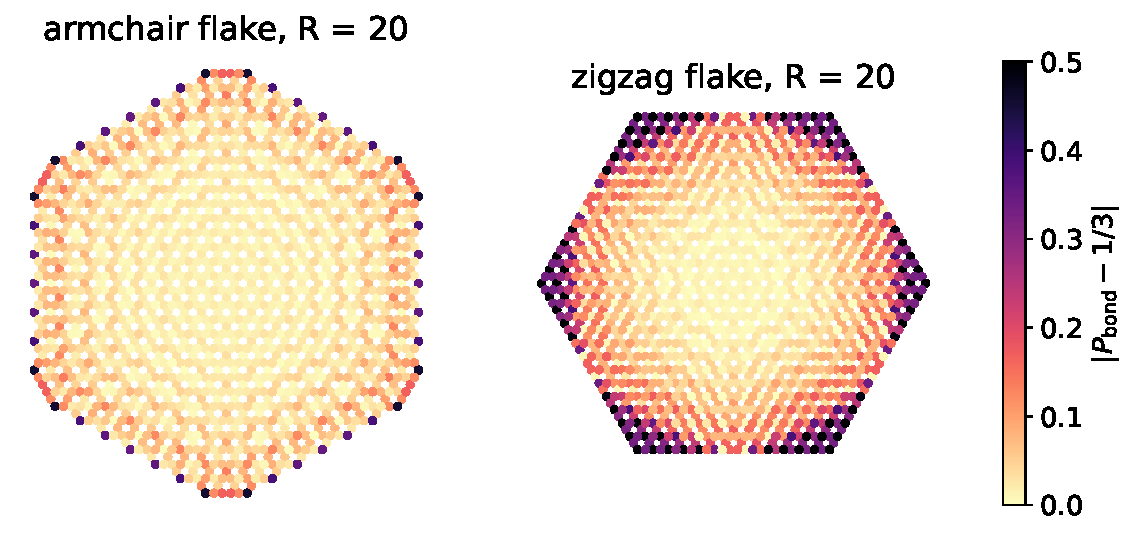
\includegraphics[width=\columnwidth]{figs/fig06_flatness.pdf}
\caption{Local deviation $|P-1/3|$ of the exact bond probabilities. Armchair flakes are flat liquids (core mean $0.035$, $0.017$, $0.012$ for $R=12,20,28$); zig-zag flakes (lozenge hexagons) freeze near the corners.}
\label{fig:flat}
\end{figure}

\begin{figure}[tbp]
\centering
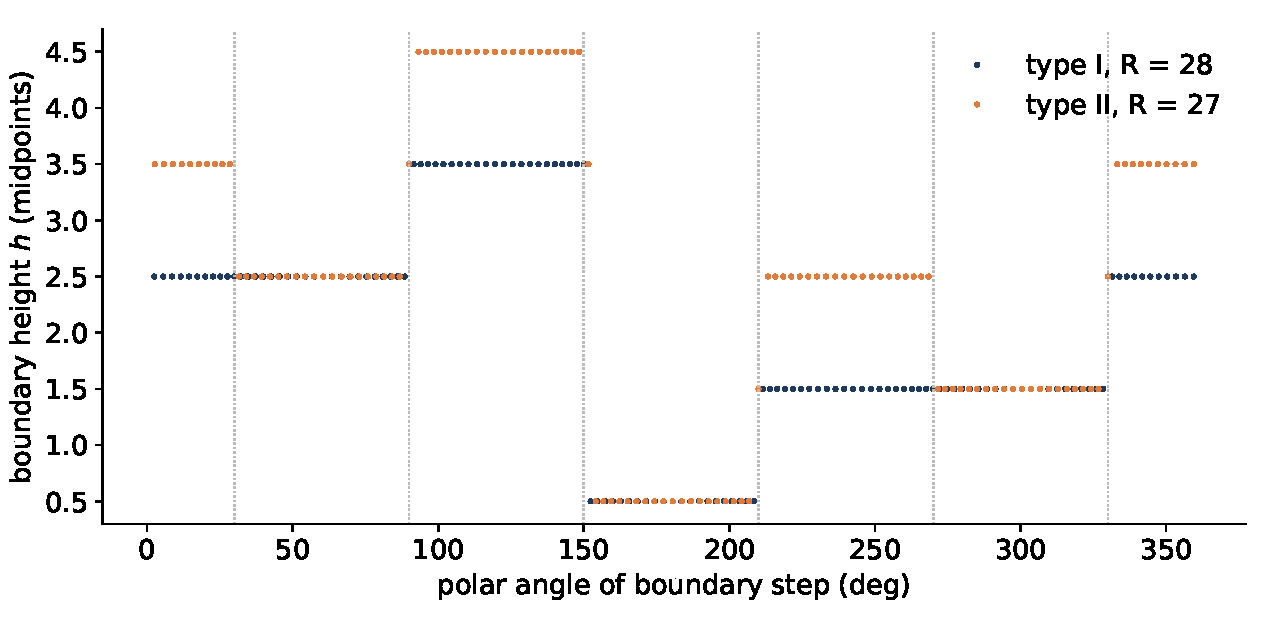
\includegraphics[width=\columnwidth]{figs/fig07_boundary_height.pdf}
\caption{Boundary height (step midpoints) around type I and type II hexagons with one forced defect. It is constant along each edge and jumps at the corners; the jump of $-3$ is the branch cut of the defect.}
\label{fig:height}
\end{figure}

\begin{figure}[tbp]
\centering
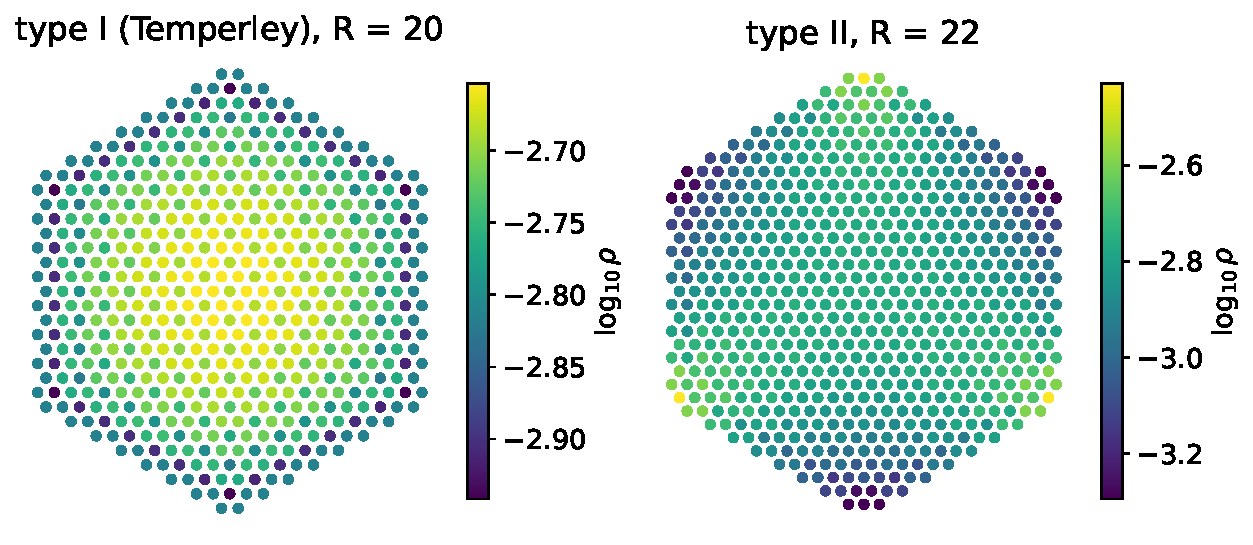
\includegraphics[width=\columnwidth]{figs/fig08_density.pdf}
\caption{Exact defect density on $A$ sites of a type I (left) and a type II (right) hexagon. Type I is Temperleyan and sixfold symmetric.}
\label{fig:density}
\end{figure}

\begin{figure*}[tbp]
\centering
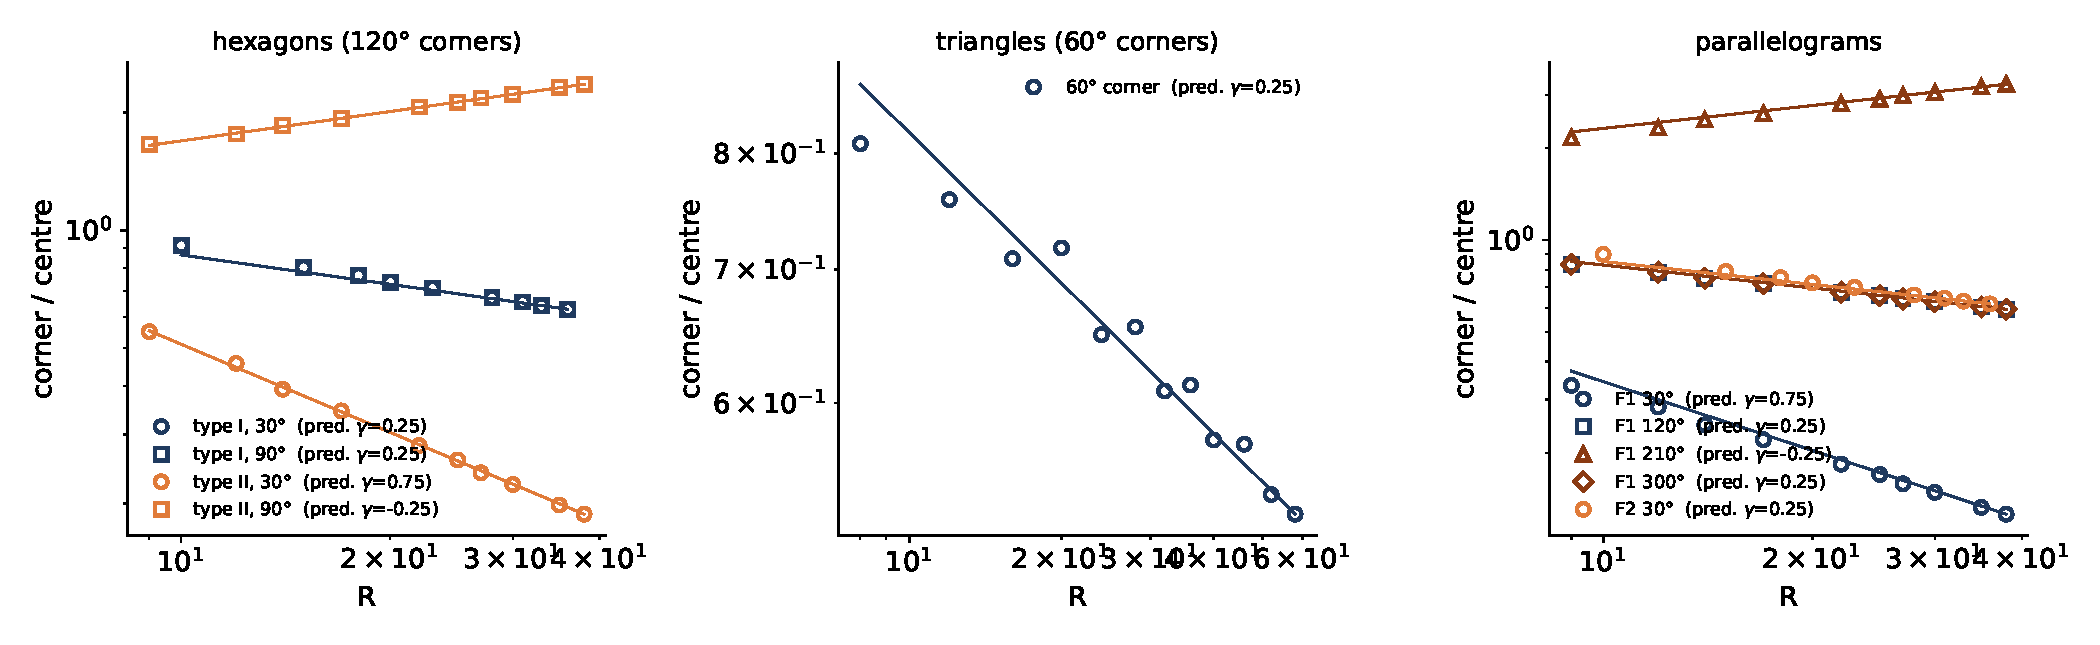
\includegraphics[width=0.98\textwidth]{figs/fig09_exponents.pdf}
\caption{Corner-to-centre ratios against size for hexagons, triangles and parallelograms. Lines have the slopes predicted by Eq.~\eqref{eq:rule}.}
\label{fig:exponents}
\end{figure*}

\emph{Independent check of the shift in finite flakes.} In balanced hexagons (no defect) the exact mean height follows from $\langle\Delta h\rangle=1-3P$ on every bond. Fitting the interior to $c+a\,u(z)$, with $u$ the harmonic function with boundary values $\pm1$ on alternating edges, gives effective jumps near the half-integers of Eq.~\eqref{eq:rule}, far from the lattice integers (Fig.~\ref{fig:Jeff}).

\begin{figure*}[tbp]
\centering
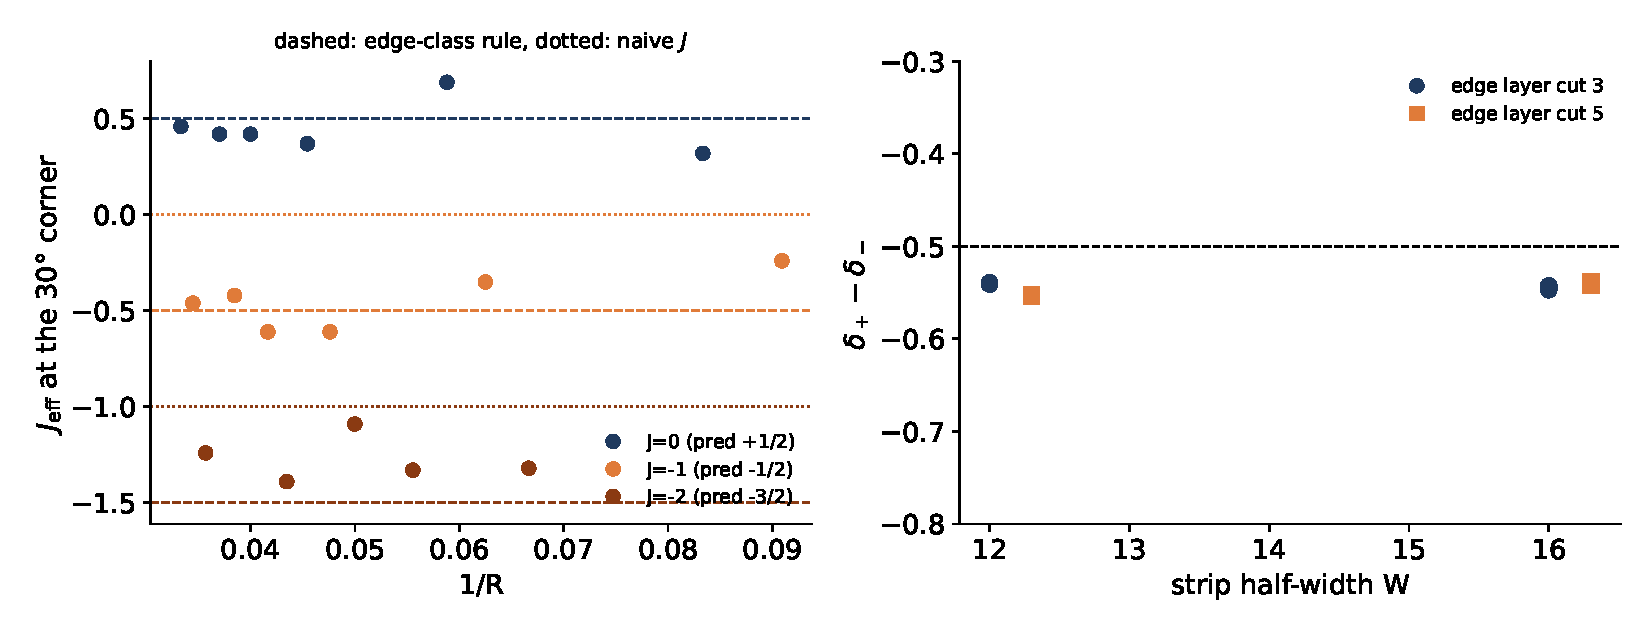
\includegraphics[width=0.8\textwidth]{figs/fig11_Jeff.pdf}
\caption{(a) Effective jump at the $30^\circ$ corner of balanced hexagons, from fits of the exact interior mean height; dashed lines are Eq.~\eqref{eq:rule}, dotted lines the lattice integers. (b) Edge-class shift from finite strips.}
\label{fig:Jeff}
\end{figure*}

\begin{figure*}[tbp]
\centering
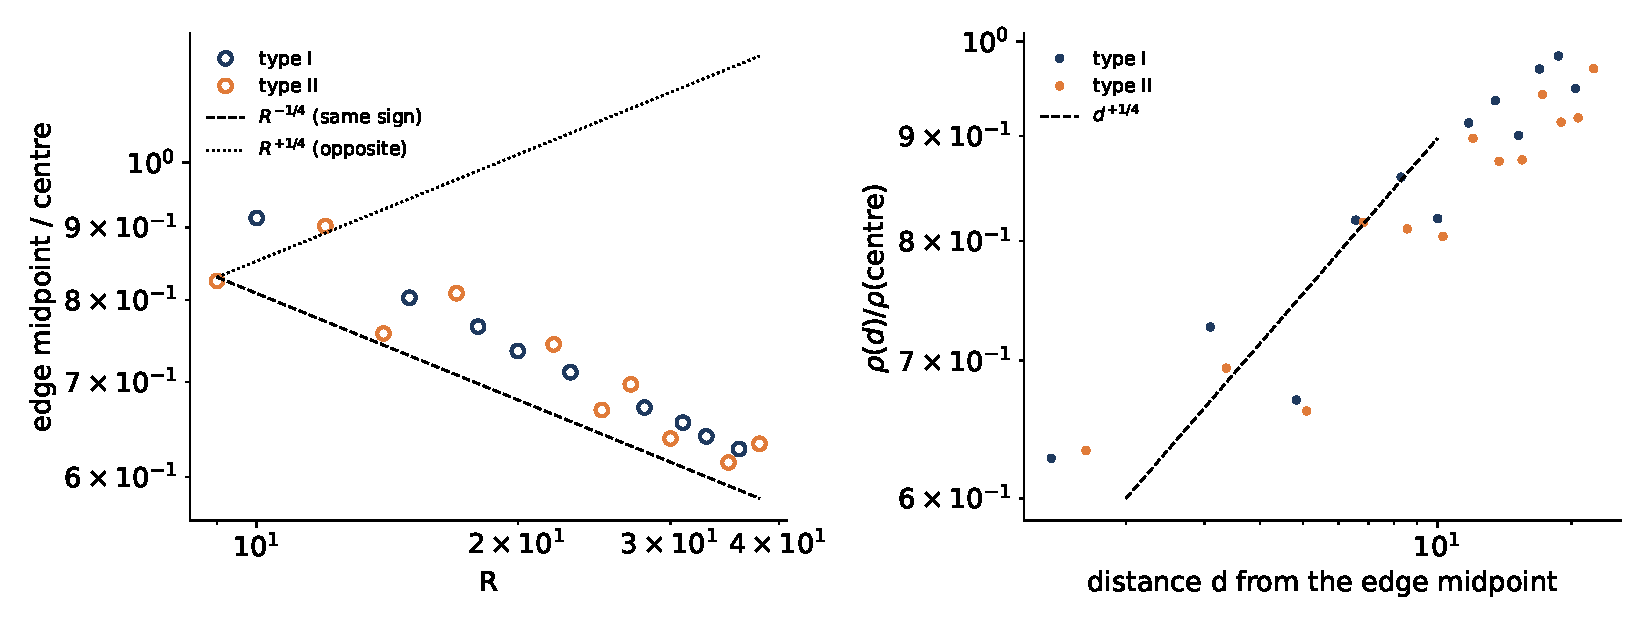
\includegraphics[width=0.8\textwidth]{figs/fig12_image.pdf}
\caption{Same-sign images on armchair edges. (a) Edge-midpoint to centre ratio against size; dashed: $R^{-1/4}$ (same sign), dotted: $R^{+1/4}$ (opposite sign). (b) Inward profile from the edge midpoint.}
\label{fig:image}
\end{figure*}

%==================================================================
\section{Diagonal model details}
\label{app:t}
%==================================================================
With a two-column unit cell the Kasteleyn symbol is $P(\theta,\varphi)=4\sin^2\varphi+|1-e^{-i\theta}-t\,e^{i\varphi}-t\,e^{-i\theta-i\varphi}|^2$, which has no zero on the unit torus for $t>0$; the perturbation gives a mass to the two Majorana fermions of the square lattice~\cite{FendleyMoessnerSondhi2002}. Figure~\ref{fig:gap}(a) shows the fermion decay rate, and Fig.~\ref{fig:gap}(b) the coefficient $a_2(N)$ of Sec.~\ref{sec:t}.

\begin{figure}[tbp]
\centering
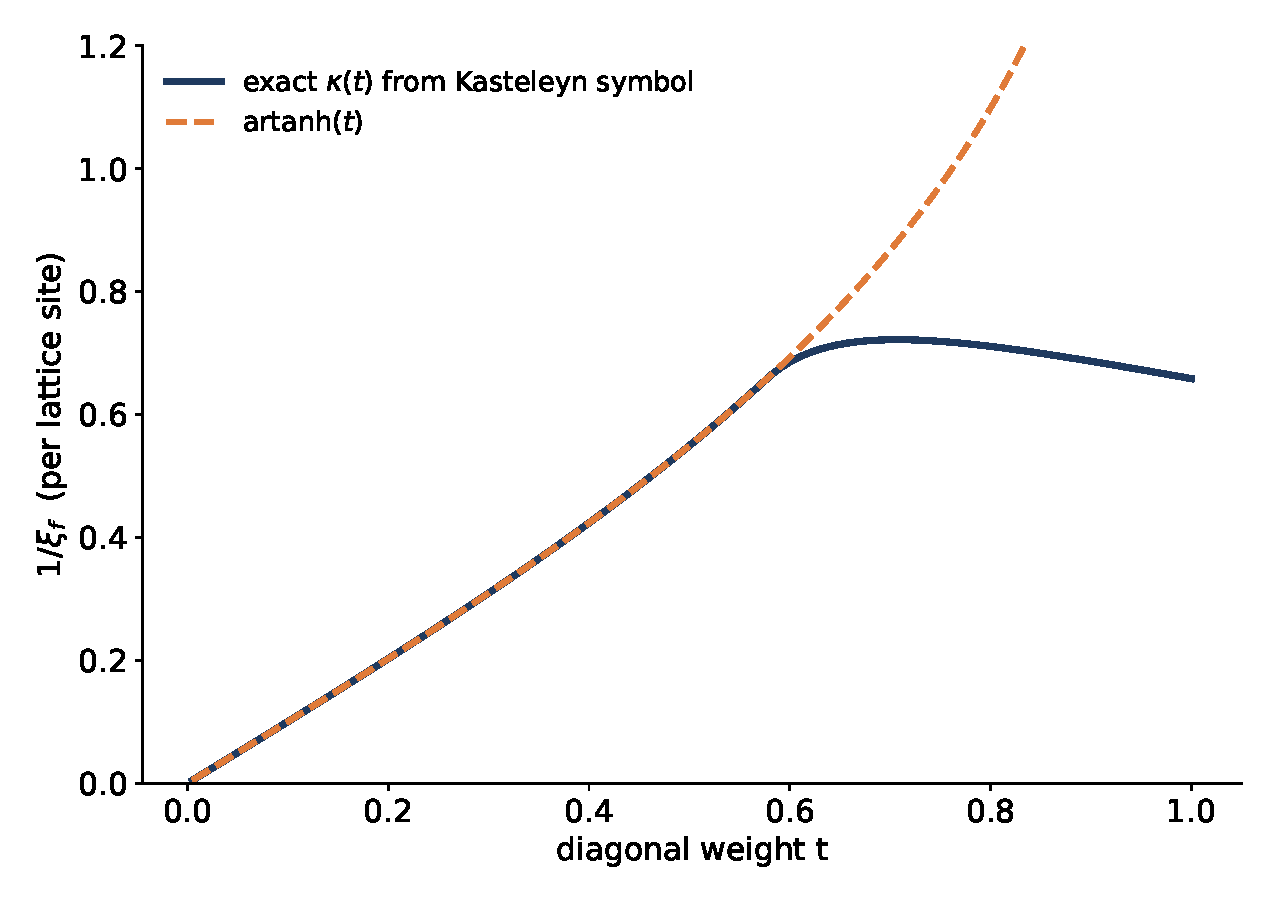
\includegraphics[width=0.49\columnwidth]{figs/fig04a_kappa.pdf}\hfill
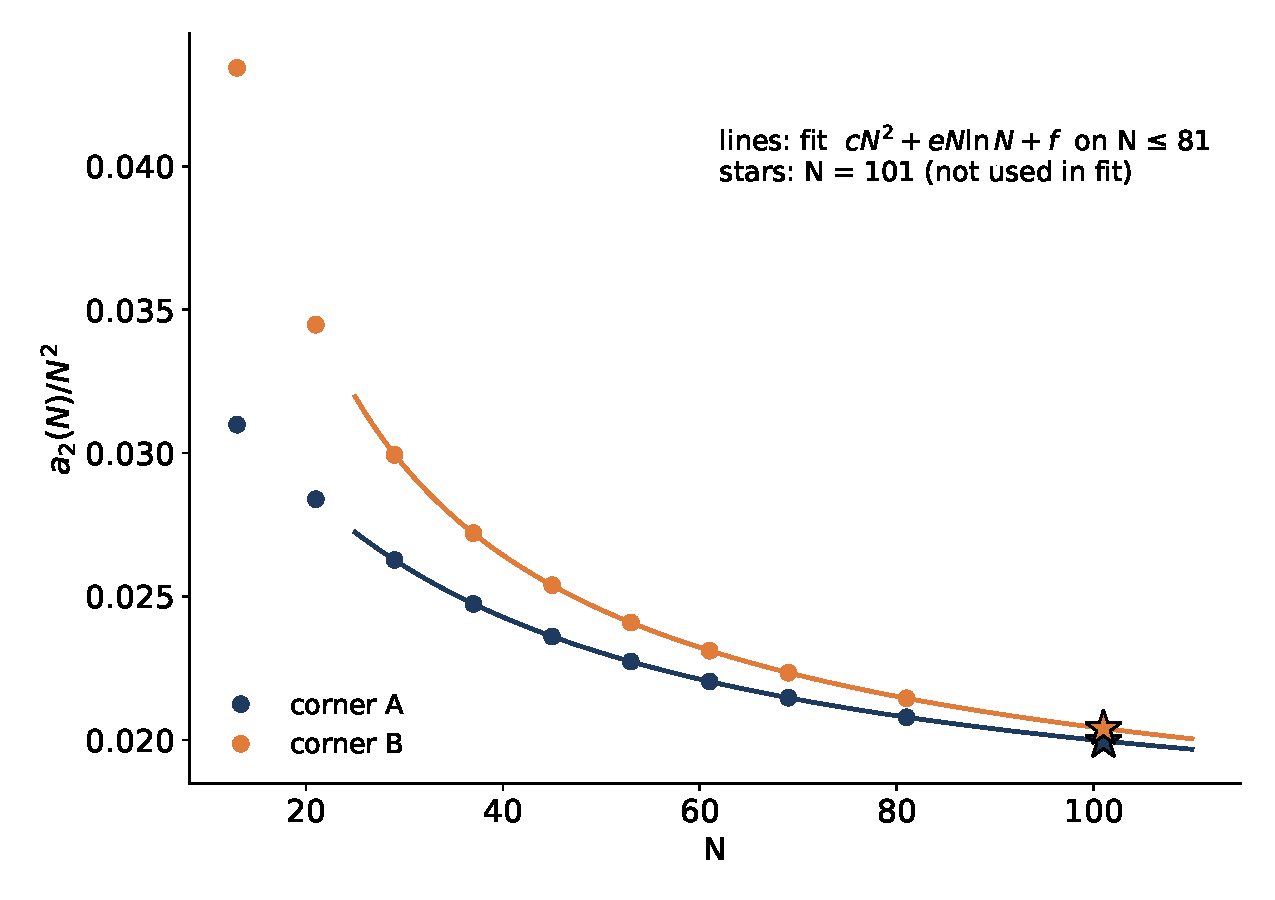
\includegraphics[width=0.49\columnwidth]{figs/fig04b_a2.pdf}
\caption{(a) Fermion decay rate from the Kasteleyn symbol and $\operatorname{artanh}t$. (b) $a_2(N)/N^2$ for both corners; lines are fits $cN^2+eN\ln N+f$ on $N\le81$, stars are $N=101$ (not used in the fit).}
\label{fig:gap}
\end{figure}

\begin{figure}[tbp]
\centering
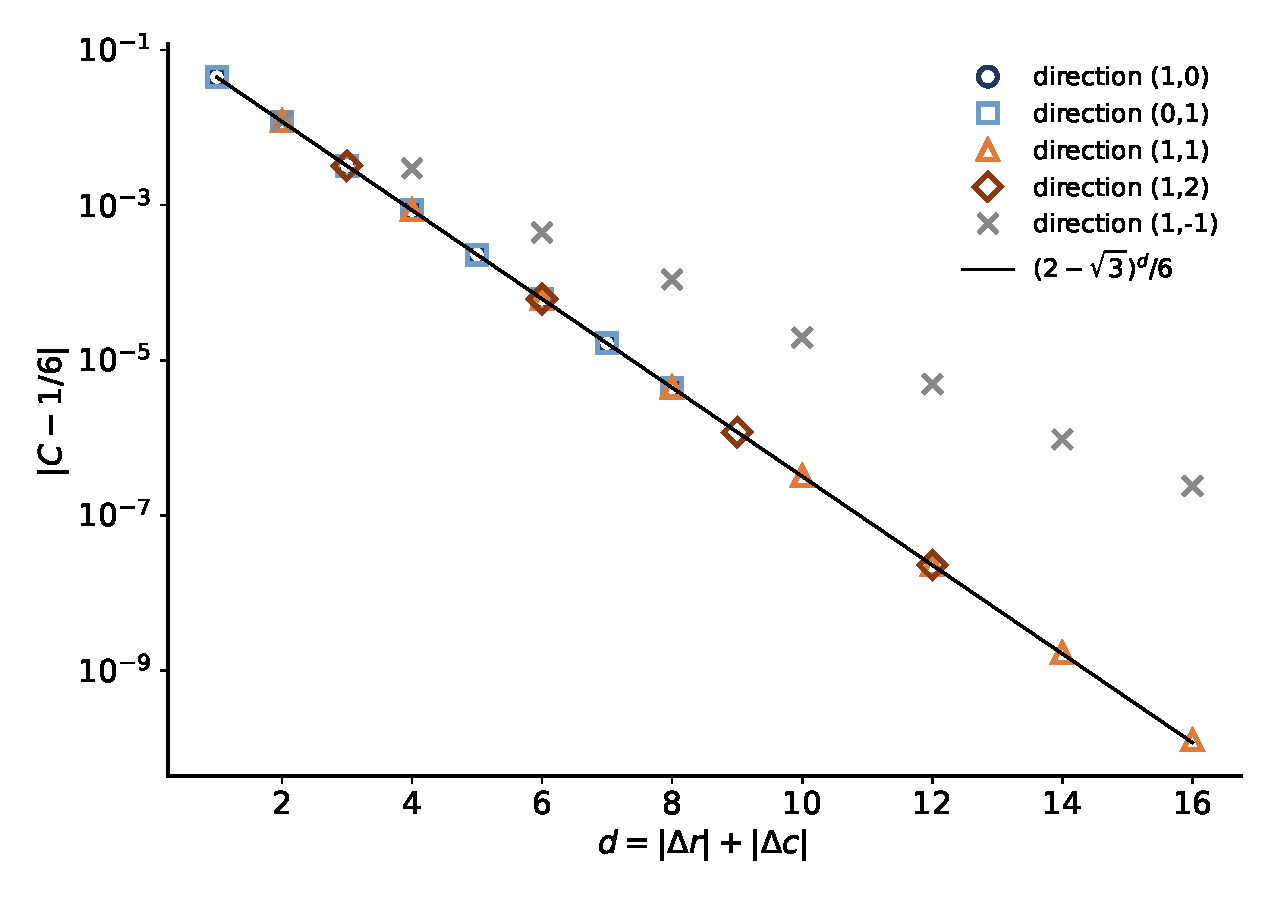
\includegraphics[width=0.85\columnwidth]{figs/fig05_half.pdf}
\caption{$|C-1/6|$ at $t=1/2$ against the Manhattan distance for several directions; the line is $(2-\sqrt3)^{d}/6$, Eq.~\eqref{eq:half}.}
\label{fig:half}
\end{figure}

Codes and data are available in the \texttt{paper2} branch of the accompanying repository.

%==================================================================
\begin{thebibliography}{99}
\bibitem{RokhsarKivelson1988} D. S. Rokhsar and S. A. Kivelson, Phys. Rev. Lett. \textbf{61}, 2376 (1988).
\bibitem{FendleyMoessnerSondhi2002} P. Fendley, R. Moessner, and S. L. Sondhi, Phys. Rev. B \textbf{66}, 214513 (2002).
\bibitem{Henley2010} C. L. Henley, Annu. Rev. Condens. Matter Phys. \textbf{1}, 179 (2010).
\bibitem{Ciucu2010} M. Ciucu, Trans. Amer. Math. Soc. \textbf{362}, 4921 (2010).
\bibitem{Ciucu2017} M. Ciucu, Proc. Amer. Math. Soc. \textbf{145}, 4931 (2017).
\bibitem{FisherStephenson1963} M. E. Fisher and J. Stephenson, Phys. Rev. \textbf{132}, 1411 (1963).
\bibitem{Kenyon2000} R. Kenyon, Ann. Probab. \textbf{28}, 759 (2000).
\bibitem{Alet2005} F. Alet, J. L. Jacobsen, G. Misguich, V. Pasquier, F. Mila, and M. Troyer, Phys. Rev. Lett. \textbf{94}, 235702 (2005).
\bibitem{Thurston1990} W. P. Thurston, Amer. Math. Monthly \textbf{97}, 757 (1990).
\bibitem{Nienhuis1984} B. Nienhuis, J. Stat. Phys. \textbf{34}, 731 (1984).
\bibitem{Kenyon2001} R. Kenyon, Ann. Probab. \textbf{29}, 1128 (2001).
\bibitem{Ciucu2014} M. Ciucu, arXiv:1202.1188.
\bibitem{Ciucu2016} M. Ciucu, Commun. Math. Phys. \textbf{344} (2016); arXiv:1405.2799.
\bibitem{CiucuKrattenthaler2011} M. Ciucu and C. Krattenthaler, Commun. Math. Phys. \textbf{302}, 253 (2011).
\bibitem{Ciucu2015} M. Ciucu, Commun. Math. Phys. \textbf{334} (2015); arXiv:1403.0925.
\bibitem{CiucuFischer2015} M. Ciucu and I. Fischer, arXiv:1405.4235.
\bibitem{PriezzhevRuelle2008} V. B. Priezzhev and P. Ruelle, Phys. Rev. E \textbf{77}, 061126 (2008).
\bibitem{Allegra2015} N. Allegra, Nucl. Phys. B \textbf{894}, 685 (2015).
\bibitem{BasorEhrhardt2007} E. L. Basor and T. Ehrhardt, Commun. Math. Phys. \textbf{274}, 427 (2007).
\bibitem{BasorBleher2016} E. Basor and P. Bleher, arXiv:1610.08021 (2016).
\bibitem{PaperI} C. Won, \emph{Electrostatics of forced defects in dimer coverings: corner charges, image charges, and boundary chemical potentials} (submitted).
\bibitem{KenyonOkounkovSheffield} R. Kenyon, A. Okounkov, and S. Sheffield, Ann. Math. \textbf{163}, 1019 (2006).
\bibitem{KenyonProppWilson} R. Kenyon, J. Propp, and D. Wilson, Electron. J. Combin. \textbf{7}, R25 (2000).
\end{thebibliography}

\end{document}
